\documentclass[]{article}
\usepackage{lmodern}
\usepackage{amssymb,amsmath}
\usepackage{ifxetex,ifluatex}
\usepackage{fixltx2e} % provides \textsubscript
\ifnum 0\ifxetex 1\fi\ifluatex 1\fi=0 % if pdftex
  \usepackage[T1]{fontenc}
  \usepackage[utf8]{inputenc}
\else % if luatex or xelatex
  \ifxetex
    \usepackage{mathspec}
  \else
    \usepackage{fontspec}
  \fi
  \defaultfontfeatures{Ligatures=TeX,Scale=MatchLowercase}
\fi
% use upquote if available, for straight quotes in verbatim environments
\IfFileExists{upquote.sty}{\usepackage{upquote}}{}
% use microtype if available
\IfFileExists{microtype.sty}{%
\usepackage[]{microtype}
\UseMicrotypeSet[protrusion]{basicmath} % disable protrusion for tt fonts
}{}
\PassOptionsToPackage{hyphens}{url} % url is loaded by hyperref
\usepackage[unicode=true]{hyperref}
\hypersetup{
            pdftitle={Comparing the Cariaco SST reconstruction to CRU data from 1900--2009},
            pdfauthor={W. Christopher Carleton},
            pdfborder={0 0 0},
            breaklinks=true}
\urlstyle{same}  % don't use monospace font for urls
\usepackage[margin=1in]{geometry}
\usepackage{color}
\usepackage{fancyvrb}
\newcommand{\VerbBar}{|}
\newcommand{\VERB}{\Verb[commandchars=\\\{\}]}
\DefineVerbatimEnvironment{Highlighting}{Verbatim}{commandchars=\\\{\}}
% Add ',fontsize=\small' for more characters per line
\usepackage{framed}
\definecolor{shadecolor}{RGB}{248,248,248}
\newenvironment{Shaded}{\begin{snugshade}}{\end{snugshade}}
\newcommand{\KeywordTok}[1]{\textcolor[rgb]{0.13,0.29,0.53}{\textbf{#1}}}
\newcommand{\DataTypeTok}[1]{\textcolor[rgb]{0.13,0.29,0.53}{#1}}
\newcommand{\DecValTok}[1]{\textcolor[rgb]{0.00,0.00,0.81}{#1}}
\newcommand{\BaseNTok}[1]{\textcolor[rgb]{0.00,0.00,0.81}{#1}}
\newcommand{\FloatTok}[1]{\textcolor[rgb]{0.00,0.00,0.81}{#1}}
\newcommand{\ConstantTok}[1]{\textcolor[rgb]{0.00,0.00,0.00}{#1}}
\newcommand{\CharTok}[1]{\textcolor[rgb]{0.31,0.60,0.02}{#1}}
\newcommand{\SpecialCharTok}[1]{\textcolor[rgb]{0.00,0.00,0.00}{#1}}
\newcommand{\StringTok}[1]{\textcolor[rgb]{0.31,0.60,0.02}{#1}}
\newcommand{\VerbatimStringTok}[1]{\textcolor[rgb]{0.31,0.60,0.02}{#1}}
\newcommand{\SpecialStringTok}[1]{\textcolor[rgb]{0.31,0.60,0.02}{#1}}
\newcommand{\ImportTok}[1]{#1}
\newcommand{\CommentTok}[1]{\textcolor[rgb]{0.56,0.35,0.01}{\textit{#1}}}
\newcommand{\DocumentationTok}[1]{\textcolor[rgb]{0.56,0.35,0.01}{\textbf{\textit{#1}}}}
\newcommand{\AnnotationTok}[1]{\textcolor[rgb]{0.56,0.35,0.01}{\textbf{\textit{#1}}}}
\newcommand{\CommentVarTok}[1]{\textcolor[rgb]{0.56,0.35,0.01}{\textbf{\textit{#1}}}}
\newcommand{\OtherTok}[1]{\textcolor[rgb]{0.56,0.35,0.01}{#1}}
\newcommand{\FunctionTok}[1]{\textcolor[rgb]{0.00,0.00,0.00}{#1}}
\newcommand{\VariableTok}[1]{\textcolor[rgb]{0.00,0.00,0.00}{#1}}
\newcommand{\ControlFlowTok}[1]{\textcolor[rgb]{0.13,0.29,0.53}{\textbf{#1}}}
\newcommand{\OperatorTok}[1]{\textcolor[rgb]{0.81,0.36,0.00}{\textbf{#1}}}
\newcommand{\BuiltInTok}[1]{#1}
\newcommand{\ExtensionTok}[1]{#1}
\newcommand{\PreprocessorTok}[1]{\textcolor[rgb]{0.56,0.35,0.01}{\textit{#1}}}
\newcommand{\AttributeTok}[1]{\textcolor[rgb]{0.77,0.63,0.00}{#1}}
\newcommand{\RegionMarkerTok}[1]{#1}
\newcommand{\InformationTok}[1]{\textcolor[rgb]{0.56,0.35,0.01}{\textbf{\textit{#1}}}}
\newcommand{\WarningTok}[1]{\textcolor[rgb]{0.56,0.35,0.01}{\textbf{\textit{#1}}}}
\newcommand{\AlertTok}[1]{\textcolor[rgb]{0.94,0.16,0.16}{#1}}
\newcommand{\ErrorTok}[1]{\textcolor[rgb]{0.64,0.00,0.00}{\textbf{#1}}}
\newcommand{\NormalTok}[1]{#1}
\usepackage{graphicx,grffile}
\makeatletter
\def\maxwidth{\ifdim\Gin@nat@width>\linewidth\linewidth\else\Gin@nat@width\fi}
\def\maxheight{\ifdim\Gin@nat@height>\textheight\textheight\else\Gin@nat@height\fi}
\makeatother
% Scale images if necessary, so that they will not overflow the page
% margins by default, and it is still possible to overwrite the defaults
% using explicit options in \includegraphics[width, height, ...]{}
\setkeys{Gin}{width=\maxwidth,height=\maxheight,keepaspectratio}
\IfFileExists{parskip.sty}{%
\usepackage{parskip}
}{% else
\setlength{\parindent}{0pt}
\setlength{\parskip}{6pt plus 2pt minus 1pt}
}
\setlength{\emergencystretch}{3em}  % prevent overfull lines
\providecommand{\tightlist}{%
  \setlength{\itemsep}{0pt}\setlength{\parskip}{0pt}}
\setcounter{secnumdepth}{0}
% Redefines (sub)paragraphs to behave more like sections
\ifx\paragraph\undefined\else
\let\oldparagraph\paragraph
\renewcommand{\paragraph}[1]{\oldparagraph{#1}\mbox{}}
\fi
\ifx\subparagraph\undefined\else
\let\oldsubparagraph\subparagraph
\renewcommand{\subparagraph}[1]{\oldsubparagraph{#1}\mbox{}}
\fi

% set default figure placement to htbp
\makeatletter
\def\fps@figure{htbp}
\makeatother


\title{Comparing the Cariaco SST reconstruction to CRU data from 1900--2009}
\author{W. Christopher Carleton}
\date{}

\begin{document}
\maketitle

\section{Objective}\label{objective}

Compare the Cariaco SST record we analyzed to Climate Research Unit
(CRU) temperature data for the instrumental period covered by both data
sets.

\section{Get CRU Data}\label{get-cru-data}

The CRU provides access to a global gridded temperature record. These
records can be accessed (after registration) at . For more information
about the data, see
\href{https://www.nature.com/articles/s41597-020-0453-3}{Harris, I.,
Osborn, T.J., Jones, P. et al. Version 4 of the CRU TS monthly
high-resolution gridded multivariate climate dataset. Sci Data 7, 109
(2020). https://doi.org/10.1038/s41597-020-0453-3}.

The Center for Environmental Data Analysis (CEDA) hosts an online data
repository and search service that we used to extract the CRU
temperature data for the Maya region. The
\href{http://wps-web1.ceda.ac.uk/submit/form?proc_id=Subsetter}{subsetting
tool} is particular useful since it can be used to select a region and
time period subset from the total CRU gridded dataset (see figure
below).

\begin{figure}
\centering
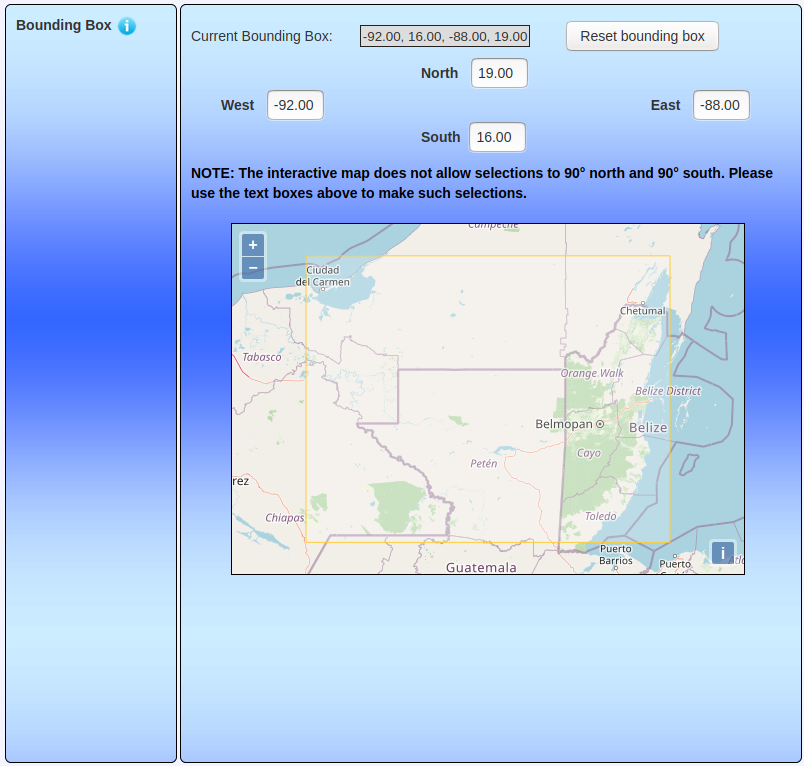
\includegraphics{../assets/img/ceda_subsetter.png}
\caption{CEDA Subsetter. Note the bounding box we selected covers most
of the Central Maya Lowlands, the core region where most of the conflict
records were discovered.}
\end{figure}

We selected an area roughly covering the Classic Maya region and
downloaded the corresponding monthly gridded temperature data. These
data are provided in multiple formats. We selected .csv format (See the
../Data folder of this archive).

Once obtained, we loaded the .csv data into an R dataframe:

\begin{Shaded}
\begin{Highlighting}[]
\NormalTok{d <-}\StringTok{ }\KeywordTok{dir}\NormalTok{(}\StringTok{"../Data/CRU/"}\NormalTok{)}
\NormalTok{d <-}\StringTok{ }\NormalTok{d[}\KeywordTok{grep}\NormalTok{(}\StringTok{"tmp"}\NormalTok{,d)]}
\NormalTok{cru <-}\StringTok{ }\KeywordTok{data.frame}\NormalTok{()}
\ControlFlowTok{for}\NormalTok{(j }\ControlFlowTok{in}\NormalTok{ d)\{}
\NormalTok{    f <-}\StringTok{ }\KeywordTok{paste}\NormalTok{(}\StringTok{"../Data/CRU/"}\NormalTok{,j,}\DataTypeTok{sep=}\StringTok{""}\NormalTok{)}
\NormalTok{    cru_tmp <-}\StringTok{ }\KeywordTok{read.csv}\NormalTok{(f,}\DataTypeTok{head=}\NormalTok{F,}\DataTypeTok{skip=}\DecValTok{44}\NormalTok{)}
\NormalTok{    cru <-}\StringTok{ }\KeywordTok{rbind}\NormalTok{(cru,cru_tmp)}
\NormalTok{\}}
\KeywordTok{head}\NormalTok{(cru)}
\end{Highlighting}
\end{Shaded}

\begin{verbatim}
##             V1    V2   V3   V4   V5   V6   V7   V8   V9
## 1 Data section 380.0   NA   NA   NA   NA   NA   NA   NA
## 2 Data section  17.4 21.7 23.1 23.5 22.3 21.1 22.6 24.2
## 3 Data section  20.1 21.0 22.7 23.2 22.1 20.7 19.9 22.9
## 4 Data section  21.6 22.3 22.9 22.9 22.0 21.9 22.0 22.8
## 5 Data section  23.3 22.9 22.6 22.4 21.8 22.0 22.6 23.1
## 6 Data section  23.2 23.0 22.5 22.2 21.6 21.4 22.3 23.0
\end{verbatim}

A bit of cleaning is required to remove non-data:

\begin{Shaded}
\begin{Highlighting}[]
\NormalTok{cru <-}\StringTok{ }\KeywordTok{as.matrix}\NormalTok{(cru[,}\OperatorTok{-}\DecValTok{1}\NormalTok{])}
\NormalTok{cru <-}\StringTok{ }\NormalTok{cru[}\KeywordTok{apply}\NormalTok{(cru,}\DecValTok{1}\NormalTok{,}\ControlFlowTok{function}\NormalTok{(x)}\KeywordTok{all}\NormalTok{(}\OperatorTok{!}\KeywordTok{is.na}\NormalTok{(x))),]}
\KeywordTok{head}\NormalTok{(cru)}
\end{Highlighting}
\end{Shaded}

\begin{verbatim}
##        V2   V3   V4   V5   V6   V7   V8   V9
## [1,] 17.4 21.7 23.1 23.5 22.3 21.1 22.6 24.2
## [2,] 20.1 21.0 22.7 23.2 22.1 20.7 19.9 22.9
## [3,] 21.6 22.3 22.9 22.9 22.0 21.9 22.0 22.8
## [4,] 23.3 22.9 22.6 22.4 21.8 22.0 22.6 23.1
## [5,] 23.2 23.0 22.5 22.2 21.6 21.4 22.3 23.0
## [6,] 23.3 23.1 22.5 22.1 21.5 21.5 22.1 22.7
\end{verbatim}

Next, we spatially averaged the CRU temperature data for the region and
created two temperature time series spanning the overlap between the CRU
data and the Cariaco SST reconstruction (i.e, 1901--2008). For one time
series, we averaged the monthly data to produce an annual average
temperature record. For the other, we included only the months
corresponding to the summer SST record, namely June, July, and August,
which produced an annual summer average record.

To create the time-series, we first need to generate spatial averages.
The rows in the cru matrix each correspond to a latitude in the gridded
dataset while the columns correspond to longitudes. There are 6 x 8 of
these grid squares in our selected study area. Since the raw data are
monthly temperatures, there are 12 of these 6-row chunks per year. Each
chunk needs to be averaged to produce the spatial average. So, we will
walk over the cru matrix in groups of 6 rows and calculate the average
of all grid-cell values in that chunk (i.e., an average of all the
values in each 6 x 8 grid):

\begin{Shaded}
\begin{Highlighting}[]
\NormalTok{month_chunks <-}\StringTok{ }\KeywordTok{seq}\NormalTok{(}\DecValTok{1}\NormalTok{,}\KeywordTok{dim}\NormalTok{(cru)[}\DecValTok{1}\NormalTok{],}\DecValTok{6}\NormalTok{)}
\NormalTok{monthly_means <-}\StringTok{ }\KeywordTok{c}\NormalTok{()}
\ControlFlowTok{for}\NormalTok{(j }\ControlFlowTok{in}\NormalTok{ month_chunks)\{}
\NormalTok{    m_tmp <-}\StringTok{ }\KeywordTok{mean}\NormalTok{(cru[j}\OperatorTok{:}\NormalTok{(j}\OperatorTok{+}\DecValTok{5}\NormalTok{),])}
\NormalTok{    monthly_means <-}\StringTok{ }\KeywordTok{c}\NormalTok{(monthly_means,m_tmp)}
\NormalTok{\}}
\end{Highlighting}
\end{Shaded}

With a vector of monthly spatial means, we can now produce both
time-series. First we produce the annual series by simply averaging
every 12 elements in the \texttt{monthly\_means} vector and then only
the rows corresponding to June, July, and August. The data we downloaded
actually corresponds to the latest CRU data and so spans 1901--2020 CE.
So, we can also remove the elements corresponding to recent years not
covered by the Cariaco SST reconstruction.

\begin{Shaded}
\begin{Highlighting}[]
\NormalTok{monthly_mean_matrix <-}\StringTok{ }\KeywordTok{matrix}\NormalTok{(monthly_means,}\DataTypeTok{nrow=}\DecValTok{12}\NormalTok{)}
\NormalTok{annual_means <-}\StringTok{ }\KeywordTok{colMeans}\NormalTok{(monthly_mean_matrix)[}\DecValTok{1}\OperatorTok{:}\DecValTok{108}\NormalTok{]}
\NormalTok{summer_means <-}\StringTok{ }\KeywordTok{colMeans}\NormalTok{(monthly_mean_matrix[}\KeywordTok{c}\NormalTok{(}\DecValTok{6}\NormalTok{,}\DecValTok{7}\NormalTok{,}\DecValTok{8}\NormalTok{),])[}\DecValTok{1}\OperatorTok{:}\DecValTok{108}\NormalTok{]}
\end{Highlighting}
\end{Shaded}

\section{Compare the records}\label{compare-the-records}

We then compared these two time-series to the Cariaco summer SST record
(\texttt{SSTRub}) with a simple linear regression.

First, we need to load the Cariaco SST record:

\begin{Shaded}
\begin{Highlighting}[]
\NormalTok{sst <-}\StringTok{ }\KeywordTok{read.csv}\NormalTok{(}\StringTok{"../Data/wurtzel2013_CariacoSST.csv"}\NormalTok{)}
\NormalTok{sst_}\DecValTok{1901}\NormalTok{_}\DecValTok{2008}\NormalTok{ <-}\StringTok{ }\KeywordTok{subset}\NormalTok{(sst,YearCE }\OperatorTok{>=}\StringTok{ }\DecValTok{1901} \OperatorTok{&}\StringTok{ }\NormalTok{YearCE }\OperatorTok{<=}\StringTok{ }\DecValTok{2008}\NormalTok{)}
\end{Highlighting}
\end{Shaded}

Then, we can aggregate all three time-series into a dataframe:

\begin{Shaded}
\begin{Highlighting}[]
\NormalTok{tempdata <-}\StringTok{ }\KeywordTok{data.frame}\NormalTok{(}
                \DataTypeTok{Year=}\DecValTok{1901}\OperatorTok{:}\DecValTok{2008}\NormalTok{,}
                \DataTypeTok{CariacoSST=}\NormalTok{sst_}\DecValTok{1901}\NormalTok{_}\DecValTok{2008}\OperatorTok{$}\NormalTok{SSTRub,}
                \DataTypeTok{CRU_Annual=}\NormalTok{annual_means,}
                \DataTypeTok{CRU_Summer=}\NormalTok{summer_means)}
\end{Highlighting}
\end{Shaded}

With this dataframe, we can now run a couple of simple linear
regressions and store the results for further analysis and plotting:

\begin{Shaded}
\begin{Highlighting}[]
\NormalTok{glm_annual <-}\StringTok{ }\KeywordTok{glm}\NormalTok{(CRU_Annual}\OperatorTok{~}\NormalTok{CariacoSST,}\DataTypeTok{data=}\NormalTok{tempdata)}
\NormalTok{glm_summer <-}\StringTok{ }\KeywordTok{glm}\NormalTok{(CRU_Summer}\OperatorTok{~}\NormalTok{CariacoSST,}\DataTypeTok{data=}\NormalTok{tempdata)}
\end{Highlighting}
\end{Shaded}

To plot the model results, we used \texttt{ggplot2}.

\begin{Shaded}
\begin{Highlighting}[]
\KeywordTok{library}\NormalTok{(ggplot2)}
\KeywordTok{library}\NormalTok{(ggpubr)}

\NormalTok{pred_annual <-}\StringTok{ }\KeywordTok{predict}\NormalTok{(glm_annual, }\DataTypeTok{se.fit=}\NormalTok{T)}
\NormalTok{pred_summer <-}\StringTok{ }\KeywordTok{predict}\NormalTok{(glm_summer, }\DataTypeTok{se.fit=}\NormalTok{T)}

\NormalTok{pred_annual_df <-}\StringTok{ }\KeywordTok{data.frame}\NormalTok{(}
                    \DataTypeTok{CariacoSST=}\NormalTok{tempdata}\OperatorTok{$}\NormalTok{CariacoSST,}
                    \DataTypeTok{GLMFit=}\NormalTok{pred_annual}\OperatorTok{$}\NormalTok{fit,}
                    \DataTypeTok{GLMSE=}\NormalTok{pred_annual}\OperatorTok{$}\NormalTok{se.fit)}

\NormalTok{pred_summer_df <-}\StringTok{ }\KeywordTok{data.frame}\NormalTok{(}
                    \DataTypeTok{CariacoSST=}\NormalTok{tempdata}\OperatorTok{$}\NormalTok{CariacoSST,}
                    \DataTypeTok{GLMFit=}\NormalTok{pred_summer}\OperatorTok{$}\NormalTok{fit,}
                    \DataTypeTok{GLMSE=}\NormalTok{pred_summer}\OperatorTok{$}\NormalTok{se.fit)}
\end{Highlighting}
\end{Shaded}

\subsection{Time Series}\label{time-series}

As always, it's useful to look at the raw data, which in this case are
the three temperature time series:

\begin{Shaded}
\begin{Highlighting}[]
\KeywordTok{ggplot}\NormalTok{(tempdata) }\OperatorTok{+}
\StringTok{    }\KeywordTok{geom_path}\NormalTok{(}\DataTypeTok{mapping=}\KeywordTok{aes}\NormalTok{(}\DataTypeTok{y=}\NormalTok{CRU_Annual,}\DataTypeTok{x=}\NormalTok{Year),}\DataTypeTok{colour=}\StringTok{"#ffbe0f"}\NormalTok{) }\OperatorTok{+}
\StringTok{    }\KeywordTok{geom_text}\NormalTok{(}
            \DataTypeTok{x=}\DecValTok{2000}\NormalTok{,}
            \DataTypeTok{y=}\KeywordTok{mean}\NormalTok{(tempdata}\OperatorTok{$}\NormalTok{CRU_Annual),}
            \DataTypeTok{colour=}\StringTok{"#ffbe0f"}\NormalTok{,}
            \DataTypeTok{label=}\StringTok{"CRU Annual"}\NormalTok{) }\OperatorTok{+}
\StringTok{    }\KeywordTok{geom_path}\NormalTok{(}\DataTypeTok{mapping=}\KeywordTok{aes}\NormalTok{(}\DataTypeTok{y=}\NormalTok{CRU_Summer,}\DataTypeTok{x=}\NormalTok{Year),}\DataTypeTok{colour=}\StringTok{"#bd2000"}\NormalTok{) }\OperatorTok{+}
\StringTok{    }\KeywordTok{geom_text}\NormalTok{(}
            \DataTypeTok{x=}\DecValTok{2000}\NormalTok{,}
            \DataTypeTok{y=}\KeywordTok{mean}\NormalTok{(tempdata}\OperatorTok{$}\NormalTok{CRU_Summer),}
            \DataTypeTok{colour=}\StringTok{"#bd2000"}\NormalTok{,}
            \DataTypeTok{label=}\StringTok{"CRU Summer"}\NormalTok{) }\OperatorTok{+}
\StringTok{    }\KeywordTok{geom_path}\NormalTok{(}\DataTypeTok{mapping=}\KeywordTok{aes}\NormalTok{(}\DataTypeTok{y=}\NormalTok{CariacoSST,}\DataTypeTok{x=}\NormalTok{Year),}\DataTypeTok{colour=}\StringTok{"#8c0000"}\NormalTok{) }\OperatorTok{+}
\StringTok{    }\KeywordTok{geom_text}\NormalTok{(}
            \DataTypeTok{x=}\DecValTok{2000}\NormalTok{,}
            \DataTypeTok{y=}\KeywordTok{mean}\NormalTok{(tempdata}\OperatorTok{$}\NormalTok{CariacoSST),}
            \DataTypeTok{colour=}\StringTok{"#8c0000"}\NormalTok{,}
            \DataTypeTok{label=}\StringTok{"Cariaco SST"}\NormalTok{) }\OperatorTok{+}
\StringTok{    }\KeywordTok{labs}\NormalTok{(}\DataTypeTok{y=}\StringTok{"Temperature (C)"}\NormalTok{, }\DataTypeTok{x=}\StringTok{"Time (CE)"}\NormalTok{) }\OperatorTok{+}
\StringTok{    }\KeywordTok{theme_minimal}\NormalTok{() }\OperatorTok{+}
\StringTok{    }\KeywordTok{theme}\NormalTok{(}\DataTypeTok{text =} \KeywordTok{element_text}\NormalTok{(}\DataTypeTok{family=}\StringTok{"Times"}\NormalTok{, }\DataTypeTok{size=}\DecValTok{12}\NormalTok{))}
\end{Highlighting}
\end{Shaded}

\begin{figure}
\centering
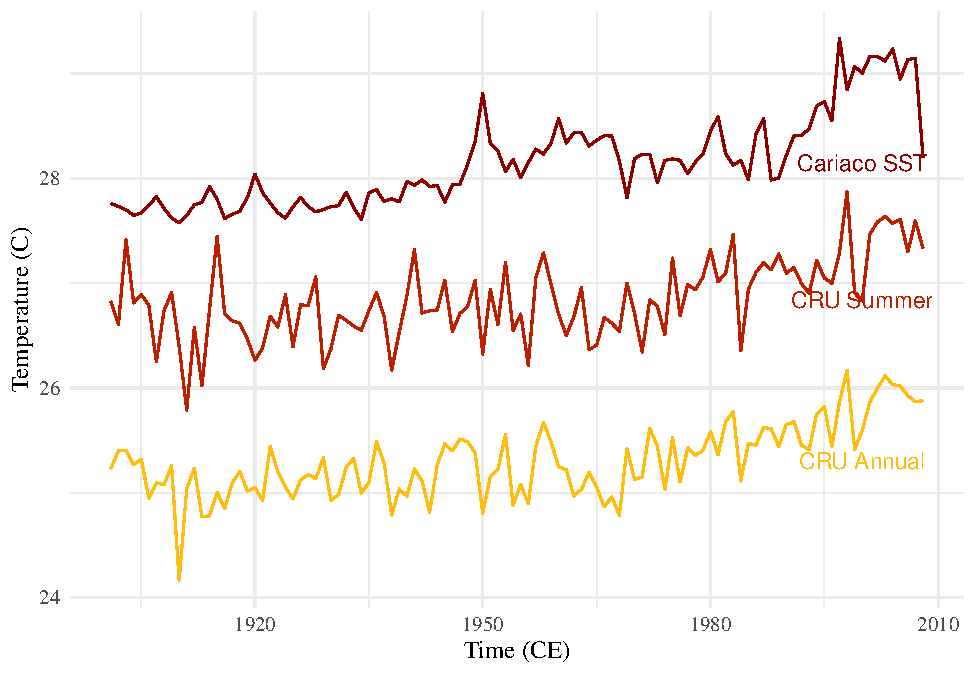
\includegraphics{cru_data_files/figure-latex/unnamed-chunk-9-1.pdf}
\caption{Temperature Time Series}
\end{figure}

\subsection{Bivariate Plots and GLM
Results}\label{bivariate-plots-and-glm-results}

Then, we can look at each of the two CRU temperature series compared to
the Cariaco reconstruction with the glm results plotted over top:

\begin{Shaded}
\begin{Highlighting}[]
\NormalTok{p1 <-}\StringTok{ }\KeywordTok{ggplot}\NormalTok{(tempdata) }\OperatorTok{+}
\StringTok{    }\KeywordTok{geom_point}\NormalTok{(}\DataTypeTok{mapping=}\KeywordTok{aes}\NormalTok{(}\DataTypeTok{y=}\NormalTok{CRU_Annual,}\DataTypeTok{x=}\NormalTok{CariacoSST),}
        \DataTypeTok{alpha=}\FloatTok{0.5}\NormalTok{) }\OperatorTok{+}
\StringTok{    }\KeywordTok{geom_path}\NormalTok{(}
        \DataTypeTok{data=}\NormalTok{pred_annual_df,}
        \DataTypeTok{mapping=}\KeywordTok{aes}\NormalTok{(}\DataTypeTok{y=}\NormalTok{GLMFit,}\DataTypeTok{x=}\NormalTok{CariacoSST),}
        \DataTypeTok{alpha=}\FloatTok{0.8}
\NormalTok{        ) }\OperatorTok{+}
\StringTok{    }\KeywordTok{geom_ribbon}\NormalTok{(}
        \DataTypeTok{data=}\NormalTok{pred_annual_df,}
        \DataTypeTok{mapping=}\KeywordTok{aes}\NormalTok{(}\DataTypeTok{x=}\NormalTok{CariacoSST,}\DataTypeTok{ymin=}\NormalTok{GLMFit }\OperatorTok{-}\StringTok{ }\NormalTok{GLMSE}\OperatorTok{*}\FloatTok{2.96}\NormalTok{,}\DataTypeTok{ymax=}\NormalTok{GLMFit }\OperatorTok{+}\StringTok{ }\NormalTok{GLMSE}\OperatorTok{*}\FloatTok{2.96}\NormalTok{),}
        \DataTypeTok{fill=}\StringTok{"steelblue"}\NormalTok{,}
        \DataTypeTok{alpha=}\FloatTok{0.5}
\NormalTok{        ) }\OperatorTok{+}
\StringTok{    }\KeywordTok{labs}\NormalTok{(}\DataTypeTok{y=}\StringTok{"Maya Region T (Annual)"}\NormalTok{, }\DataTypeTok{x=}\StringTok{"Cariaco T"}\NormalTok{) }\OperatorTok{+}
\StringTok{    }\KeywordTok{theme_minimal}\NormalTok{() }\OperatorTok{+}
\StringTok{    }\KeywordTok{theme}\NormalTok{(}\DataTypeTok{text =} \KeywordTok{element_text}\NormalTok{(}\DataTypeTok{family=}\StringTok{"Times"}\NormalTok{, }\DataTypeTok{size=}\DecValTok{12}\NormalTok{),}
        \DataTypeTok{axis.title.x=}\KeywordTok{element_blank}\NormalTok{(),}
        \DataTypeTok{axis.text.x=}\KeywordTok{element_blank}\NormalTok{(),}
        \DataTypeTok{axis.ticks.x=}\KeywordTok{element_blank}\NormalTok{())}

\NormalTok{p2 <-}\StringTok{ }\KeywordTok{ggplot}\NormalTok{(tempdata) }\OperatorTok{+}
\StringTok{    }\KeywordTok{geom_point}\NormalTok{(}\DataTypeTok{mapping=}\KeywordTok{aes}\NormalTok{(}\DataTypeTok{y=}\NormalTok{CRU_Summer,}\DataTypeTok{x=}\NormalTok{CariacoSST),}
        \DataTypeTok{alpha=}\FloatTok{0.5}\NormalTok{) }\OperatorTok{+}
\StringTok{    }\KeywordTok{geom_path}\NormalTok{(}
        \DataTypeTok{data=}\NormalTok{pred_summer_df,}
        \DataTypeTok{mapping=}\KeywordTok{aes}\NormalTok{(}\DataTypeTok{y=}\NormalTok{GLMFit,}\DataTypeTok{x=}\NormalTok{CariacoSST),}
        \DataTypeTok{alpha=}\FloatTok{0.8}
\NormalTok{        ) }\OperatorTok{+}
\StringTok{    }\KeywordTok{geom_ribbon}\NormalTok{(}
        \DataTypeTok{data=}\NormalTok{pred_summer_df,}
        \DataTypeTok{mapping=}\KeywordTok{aes}\NormalTok{(}\DataTypeTok{x=}\NormalTok{CariacoSST,}\DataTypeTok{ymin=}\NormalTok{GLMFit }\OperatorTok{-}\StringTok{ }\NormalTok{GLMSE}\OperatorTok{*}\FloatTok{2.96}\NormalTok{,}\DataTypeTok{ymax=}\NormalTok{GLMFit }\OperatorTok{+}\StringTok{ }\NormalTok{GLMSE}\OperatorTok{*}\FloatTok{2.96}\NormalTok{),}
        \DataTypeTok{fill=}\StringTok{"steelblue"}\NormalTok{,}
        \DataTypeTok{alpha=}\FloatTok{0.5}
\NormalTok{        ) }\OperatorTok{+}
\StringTok{    }\KeywordTok{labs}\NormalTok{(}\DataTypeTok{y=}\StringTok{"Maya Region T (Summer)"}\NormalTok{, }\DataTypeTok{x=}\StringTok{"Cariaco T"}\NormalTok{) }\OperatorTok{+}
\StringTok{    }\KeywordTok{theme_minimal}\NormalTok{() }\OperatorTok{+}
\StringTok{    }\KeywordTok{theme}\NormalTok{(}\DataTypeTok{text =} \KeywordTok{element_text}\NormalTok{(}\DataTypeTok{family=}\StringTok{"Times"}\NormalTok{, }\DataTypeTok{size=}\DecValTok{12}\NormalTok{))}

\KeywordTok{ggarrange}\NormalTok{(p1,p2,}
    \DataTypeTok{ncol=}\DecValTok{1}\NormalTok{,}
    \DataTypeTok{nrow=}\DecValTok{2}\NormalTok{,}
    \DataTypeTok{align=}\StringTok{"v"}\NormalTok{)}
\end{Highlighting}
\end{Shaded}

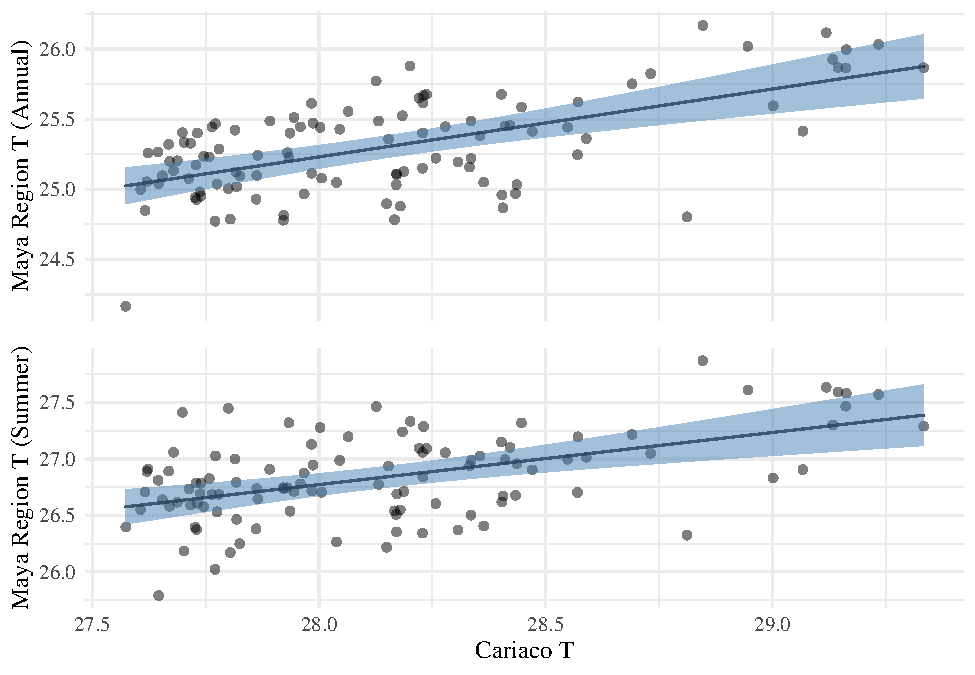
\includegraphics{cru_data_files/figure-latex/unnamed-chunk-10-1.pdf}

\subsection{Effects}\label{effects}

We can also display the regression results numerically:

\begin{Shaded}
\begin{Highlighting}[]
\KeywordTok{summary}\NormalTok{(glm_annual)}
\end{Highlighting}
\end{Shaded}

\begin{verbatim}
## 
## Call:
## glm(formula = CRU_Annual ~ CariacoSST, data = tempdata)
## 
## Deviance Residuals: 
##      Min        1Q    Median        3Q       Max  
## -0.85884  -0.17676   0.03006   0.20687   0.55137  
## 
## Coefficients:
##             Estimate Std. Error t value Pr(>|t|)    
## (Intercept)  11.6871     1.7087   6.840 5.27e-10 ***
## CariacoSST    0.4837     0.0607   7.968 1.95e-12 ***
## ---
## Signif. codes:  0 '***' 0.001 '**' 0.01 '*' 0.05 '.' 0.1 ' ' 1
## 
## (Dispersion parameter for gaussian family taken to be 0.07527857)
## 
##     Null deviance: 12.7594  on 107  degrees of freedom
## Residual deviance:  7.9795  on 106  degrees of freedom
## AIC: 31.124
## 
## Number of Fisher Scoring iterations: 2
\end{verbatim}

\begin{Shaded}
\begin{Highlighting}[]
\KeywordTok{summary}\NormalTok{(glm_summer)}
\end{Highlighting}
\end{Shaded}

\begin{verbatim}
## 
## Call:
## glm(formula = CRU_Summer ~ CariacoSST, data = tempdata)
## 
## Deviance Residuals: 
##      Min        1Q    Median        3Q       Max  
## -0.82356  -0.21154   0.01089   0.19201   0.77889  
## 
## Coefficients:
##             Estimate Std. Error t value Pr(>|t|)    
## (Intercept) 13.84829    2.03422   6.808 6.16e-10 ***
## CariacoSST   0.46158    0.07227   6.387 4.59e-09 ***
## ---
## Signif. codes:  0 '***' 0.001 '**' 0.01 '*' 0.05 '.' 0.1 ' ' 1
## 
## (Dispersion parameter for gaussian family taken to be 0.1066938)
## 
##     Null deviance: 15.662  on 107  degrees of freedom
## Residual deviance: 11.310  on 106  degrees of freedom
## AIC: 68.79
## 
## Number of Fisher Scoring iterations: 2
\end{verbatim}

\end{document}
